\documentclass[a4paper,12pt]{report}
\usepackage[utf8]{inputenc}
\usepackage[T1]{fontenc}
\usepackage[francais]{babel}
\usepackage{graphicx}  %image hda text
\usepackage{wrapfig} %pour les image
\usepackage{subcaption} %pour groupe images
\usepackage[final]{pdfpages}  %include pdf
\usepackage{textcomp} 
\usepackage{mathtools}
\usepackage{amssymb}
\usepackage{amsmath}
\usepackage[
  top=1in,
  bottom=1in,
  left=1in,
  right=1in,
  footskip=0.5in,
  headheight=16pt
  ]{geometry}
 \DeclareUnicodeCharacter{202F}{\,} 
\usepackage{fancyhdr}
\pagestyle{fancy}
\fancyhf{}

\fancyhead[RE,LO]{\rightmark} % section title in header 
\fancyfoot[CE,CO]{\thepage}	 % page number


\usepackage{color} 

\usepackage{hyperref} 
\hypersetup{
    colorlinks=true,
    linktoc=all,
    linkcolor=black,
    urlcolor=blue
}


\begin{document}


\begin{wrapfigure}[2]{r}{2cm}
\vspace{-5 pt}

\includegraphics[width=2.5cm]{img/logo.jpg}
\centering
\end{wrapfigure}
 \textbf{\scriptsize UNIVERSITE DES SCIENCESET DE LA TECHNOLOGIE D’ORAN-USTOMB-  }\\ \\
 \textbf{\footnotesize
 Faculté des Mathemathiques et Informatiques \\
 Departement Informatique 
}
  \\[1.5cm]
\newcommand{\HRule}{\rule{\linewidth}{0.5mm}}

\begin{center}
\vfill

\HRule \\[0.6cm]

{\huge\bfseries{\color{blue}{MARIAGE STABLE : MATCH-UP}} \\[0.25cm]}
\HRule \\[1.5cm]
\vfill

\vfill
\vfill


\vfill
\large{  Projet  présenté par : } \\
Atelier 1 

\vfill

\large{Spécialité :} \\
SID\\
Groupe : 01
\vfill
\bigskip


\vfill

 \vfill
       
     \vfill

année universitaire: 2020-2021
 \end{center}

 

\chapter{Le Problème du Mariage Homme/Femme}
\begin{abstract}

\par L'objectif principal de cette section est de présenter l'algorithme  originel de Gale et Shapley, décrit dans le cadre imagé du mariage. Nous montrerons que cet algorithme permet dans une large mesure de définir un mécanisme d’appariement satisfaisant, qui réponde à trois exigences : stabilité, optimalité et absence de manipulation 
 Les résultats présentés témoigneront de la robustesse du mécanisme dérivé de l’algorithme, bien au-delà du cadre initial de Gale et Shapley [1962], qui n’envisageait pas de comportement stratégique de la part des individus à marier. 
\cite{abstract}
\end{abstract}
  
\tableofcontents
\listoffigures 
\newpage
\section{Introduction}
	\par Le problème du mariage stable indique qu'étant donné N hommes et N femmes, où chaque personne a classé tous les membres du sexe opposé par ordre de préférence, marier les hommes et les femmes ensemble de telle sorte qu'il n'y ait pas deux personnes de sexe opposé qui préféreraient toutes les deux entre eux que leurs partenaires actuels. S'il n'y a pas de telles personnes, tous les mariages sont « stables ». \cite{intro_algo}
	
		\begin{flushleft}
		\textbf{la question qui se pose ... }
		\end{flushleft}
		\vspace{4cm}
	\begin{center}
		\textit{EST CE QUE IL Y A DES THÉORIES OU DES ALGORITHMES TRAIENT CE GENRE DE PROBLÈME ?}
	\end{center}
\newpage

\section{Théorie de jeux}
\par La théorie des jeux est un domaine des mathématiques qui s'intéresse aux interactions stratégiques des agents (appelés « joueurs »). Les fondements mathématiques de la théorie moderne des jeux sont décrits autour des années 1920 par "Ernst Zermelo" . Ces idées sont ensuite développées par Oskar Morgenstern et John von Neumann en 1944 dans leur ouvrage Theory of Games and Economic Behavior qui est considéré comme le fondement de la théorie des jeux moderne. Il s'agissait de modéliser les jeux à somme nulle où la somme des gains entre les joueurs est toujours égale à zéro. La théorie des jeux devient dès ce moment un outil théorique important de la microéconomie.\cite{tj}

\section{Le problème des mariages stables}

 	\subsection{définition}
 		\par On dit qu’une femme est possible pour un homme s’il existe au moins un couplage stable pour lequel cette femme et cet homme sont en couple. Sinon, on dit que cette femme est impossible pour cet homme.
De même, on définit un homme possible et impossible pour une femme.
\par On peut monter avec un exemple simple qu’il n’existe pas toujours une solution satisfaisant à la fois les hommes et les femmes : on a deux hommes  $ \alpha $ et $\beta$ et deux femmes A et B tels que $\alpha$ préfère A,$\beta$ préfère B, A préfère $\beta$ et B préfère $\alpha$.	
 \begin{figure}[h!]
	\center
	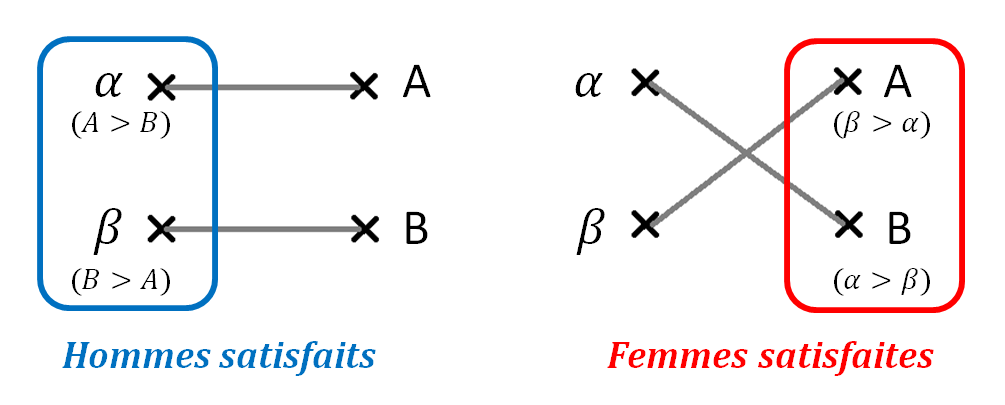
\includegraphics[scale=0.6]{img/def.png}
	\caption{schéma de satisfaction}
	
\end{figure}

\par Dans cette situation, une solution favorisera toujours les hommes au dépend des femmes ou les femmes au dépend des hommes.	
\cite{def}
\section{Algorithme de Gale-Shapley }
\subsection{Qui sont Gale and Shapley?}
\subsubsection{Lloyd Shapley} Lloyd Stowell Shapley (2 juin 1923 à Cambridge au Massachusetts - 12 mars 2016 à Tucson dans l'Arizona) est un \textbf{mathématicien} et \textbf{économiste} américain. Il est professeur émérite à l’université de Californie à Los Angeles (UCLA). Il a contribué aux domaines de l’économie mathématique et surtout de la \textbf{théorie des jeux}. Lloyd Shapley est considéré par de nombreux experts comme le plus grand théoricien des jeux depuis les travaux de Von Neumann et Morgenstern en 1940. Il est co-lauréat avec Alvin Roth du prix dit Nobel d'économie en 2012 « pour la théorie des allocations stables et la pratique de la conception de marchés » \cite{Shapley}
\subsubsection{David Gale}
\par David Gale est un mathématicien et économiste américain né le 13 décembre 1921 à New York et décédé le 7 mars 2008 à Berkeley. Il est professeur émérite à l'université de Californie à Berkeley. Il est connu pour son article commun avec Lloyd Shapley sur l'équilibre d'un modèle d'appariement optimal et l'application au problème de l'admission à l'université et de la formation des couples. \cite{David_Gale}
\subsection{L'algorithme}
Considérez l'exemple suivant.
\begin{itemize}
\item Let there be two men m1 and m2 and two women w1 and w2. 
\begin{itemize}
\item Soit la liste des préférences de m1 {w1, w2}
\item Soit la liste des préférences de m2 {w1, w2}
\item Soit la liste des préférences de w1 {m1, m2}
\item  Soit la liste des préférences de w2 {m1, m2}
\end{itemize}
\end{itemize}

L'appariement { {m1, w2}, {w1, m2} } n'est pas stable car m1 et w1 se préféreraient à leurs partenaires assignés. L'appariement {m1, w1} et {m2, w2} est stable car il n'y a pas deux personnes de sexe opposé qui se préféreraient à leurs partenaires assignés.
Il est toujours possible de former des mariages stables à partir de listes de préférences. Voici l'algorithme Gale-Shapley pour trouver une correspondance stable :
L'idée est de parcourir tous les hommes libres tant qu'il n'y a aucun homme libre disponible. Chaque homme libre va vers toutes les femmes de sa liste de préférences selon l'ordre. Pour chaque femme qu'il fréquente, il vérifie si la femme est libre, si oui, ils se fiancent tous les deux. Si la femme n'est pas libre, alors la femme choisit soit de lui dire non, soit d'abandonner son engagement actuel en fonction de sa liste de préférences. Ainsi, un engagement fait une fois peut être rompu si une femme obtient une meilleure option. La complexité temporelle de l'algorithme Gale-Shapley est O(n2).

\begin{figure}[h!]
	\center
	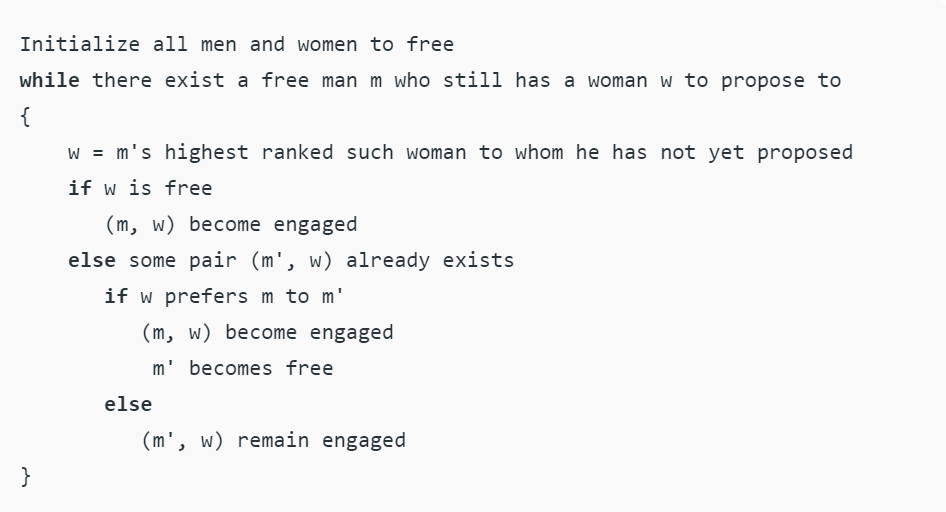
\includegraphics[scale=0.7]{img/algo.png}
	\caption{Algorithme de Gale-Shapley }
	
\end{figure}


\subsubsection{Stabilité}
 \par L’un des objectifs annoncés par Gale et Shapley est d’étudier la « stabilité » des mariages qui résultent de leur algorithme. Leur concept de stabilité repose sur deux conditions minimales.
 \\
 Gale et Shapley [1962] Dans tout modèle de mariage, quelles que soient les préférences des individus, il existe un appariement stable. Plus précisément, l’appariement résultant de l’algorithme d’acceptation différée, en faveur des hommes, est stable (et de même pour l’algorithme en faveur des femmes).
 \\
La preuve du résultat suit immédiatement de deux propriétés de l’algorithme d’acceptation différée. Premièrement, l’algorithme produit un appariement qui n’associe jamais un homme et une femme qui ne soient pas mutuellement acceptables, de sorte que l’appariement final est individuellement rationnel. Deuxièmement, si un homme n’est pas apparié à une femme qu’il préfère à son partenaire dans l’appariement, il a nécessairement fait une proposition à cette femme à une certaine étape de l’algorithme et a été rejeté ensuite par la femme, qui a accepté l’offre d’un partenaire qu’elle classait mieux. Ce couple ne peut donc pas bloquer l’appariement. 
\subsubsection{Structure des appariements stables et optimalité}
\par Une analyse plus approfondie de l'algorithme suggère un deuxième résultat, plus fort que le premier. Gale et Shapley observent que le choix du type d'individus qui fait des propositions joue un rôle clé dans l’appariement final produit par l'algorithme. Le modèle d’appariement suppose seulement que chaque individu a une préférence sur ses partenaires possibles, mais il est très facile d’en déduire des préférences sur les appariements : un individu préfère un appariement $\mu$ à un appariement $\mu$ ' s’il préfère son partenaire dans $\mu$ à son partenaire dans $\mu$ ' . Gale et Shapley montrent que, pour les individus qui font des propositions dans l’algorithme, leur appariement correspond à un élément maximal (au sens de ces préférences induites) de l’ensemble des appariements stables.
\\ 
\par L’exemple suivant donne une illustration simple de la structure des appariements, en montrant en particulier comment les appariements sont ordonnés, selon les préférences des agents 
\begin{figure}[h!]
	\center
	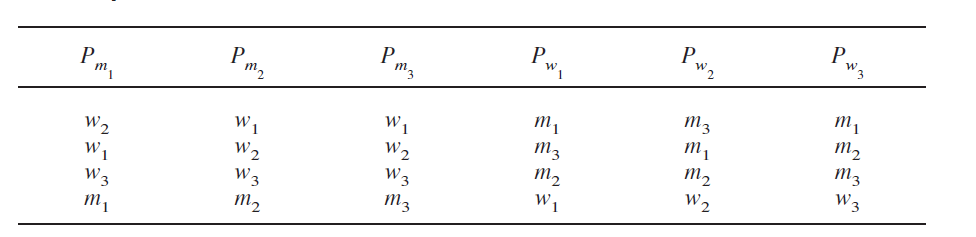
\includegraphics[scale=0.7]{img/exemple.png}
	\caption{exemple de algorithm Gale et Shapley }
	
\end{figure}
\par Il existe 2 appariements stables :

\begin{figure}[h!]
	\center
	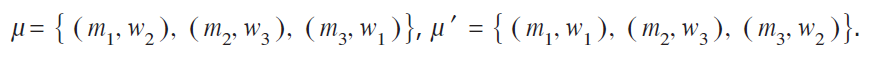
\includegraphics[scale=0.7]{img/inst.png}
	
\end{figure}

Chaque homme préfère son partenaire dans $\mu$ à son partenaire dans $\mu$ ' (et inversement pour chaque femme), w2 et w3 étant toute fois indifférents entre les deux appariements. L’appariement de Gale et Shapley en faveur des hommes correspond à $\mu$, celui des femmes est donné par $\mu$ ' .
\cite{abstract}

\section{Implémentation}
\par voir le fichier python accompagnée avec ce document
\\
"/implementation/Untitled.ipynb"
\newpage
\section{conclusion}
\par La perspective adoptée dans sa théorie économique du mariage, qui s'applique plutôt d'ailleurs à la mise en couple qu'à l'institution du mariage en elle-même, est la même que dans la théorie économique en général : les décisions en matière de mariage comme de divorce sont celles prises par des individus rationnels qui visent à maximiser leur utilité. En premier lieu, étant donné que le mariage est pratiquement toujours un acte volontaire des mariés ou de leurs parents, la théorie économique des préférences montre que les personnes qui se marient espèrent élever leur niveau d’utilité au-dessus de ce qu’il serait s’ils restaient célibataires.
\\ 
\par On peut plus précisément considérer le mariage (ou, plus généralement, la vie en couple) comme un partenariat visant à réaliser à la fois une consommation et une production jointes. La production la plus évidente est, bien entendu, la mise au monde et l'éducation des enfants. Trois autres avantages économiques de la vie en couple méritent d’être mentionnés. Se fondant sur la répartition des tâches dans la famille traditionnelle (homme au travail, femme au foyer), Becker met en évidence la division du travail, qui permet de bénéficier d'économies d'échelle et d'exploiter des avantages comparatifs – son argument perd néanmoins en pertinence dans la société contemporaine. Ensuite, les mariés peuvent jouir de biens collectifs, tels que le logement, le chauffage, l’électricité (ou plus évidemment les enfants, si l’on ose les considérer comme des biens collectifs). Enfin, ils partagent des risques, comme le chômage ou la maladie.\cite{conclusion}


\bibliographystyle{plain}

\bibliography{Bibliographie}




\end{document}
